\section*{Matériel} \label{sec:Matériel}
\addcontentsline{toc}{section}{Matériel}

Ce jeu est composé de:
\begin{itemize}
\item 18x \jetonsObstacles, recto verso, répartis en 6 couleurs ( 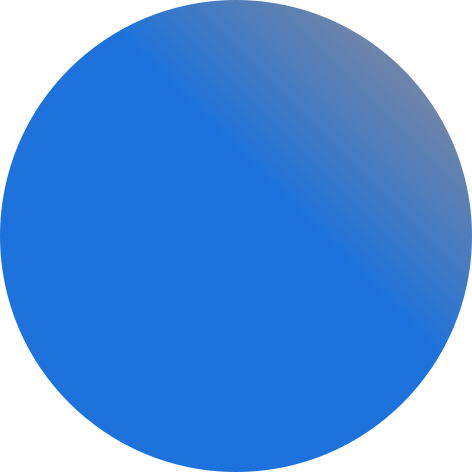
\includegraphics[scale=0.15]{obstacles/fond_bleu}, 
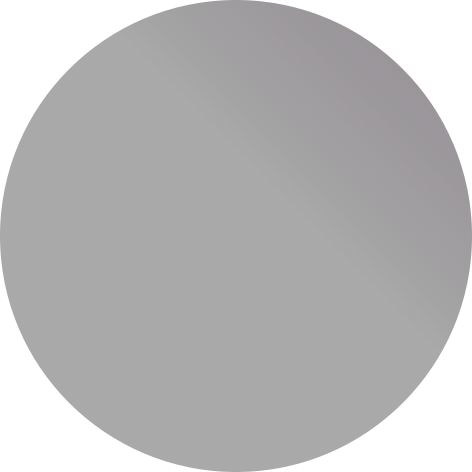
\includegraphics[scale=0.15]{obstacles/fond_gris}, 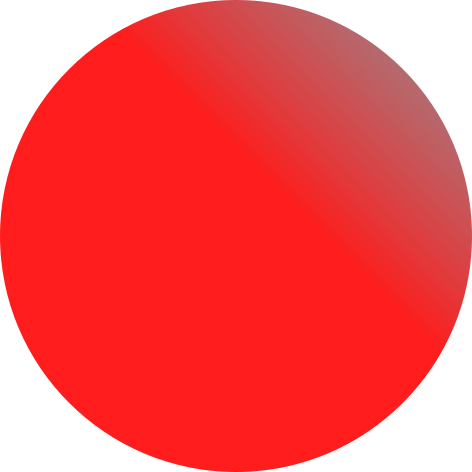
\includegraphics[scale=0.15]{obstacles/fond_rouge}, 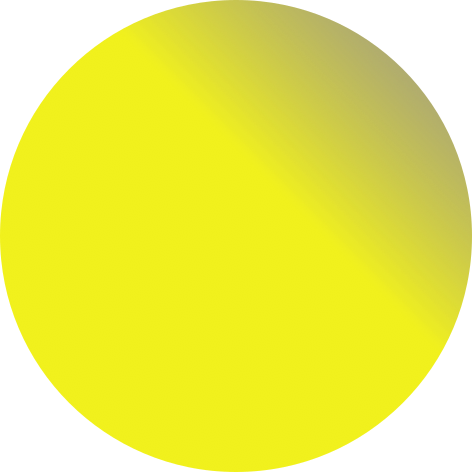
\includegraphics[scale=0.15]{obstacles/fond_jaune}, 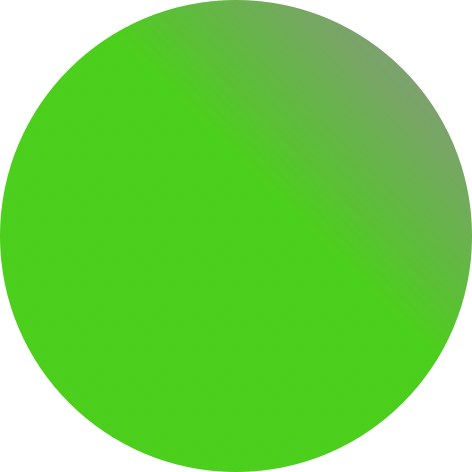
\includegraphics[scale=0.15]{obstacles/fond_vert}, 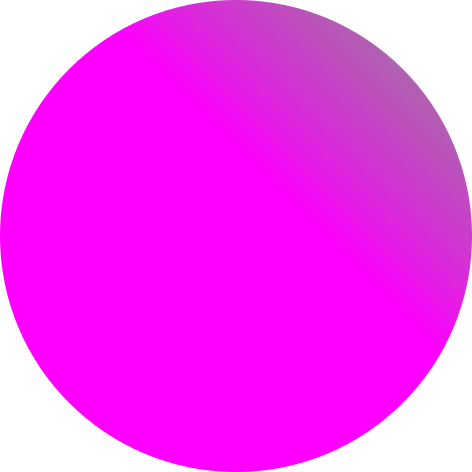
\includegraphics[scale=0.15]{obstacles/fond_violet} ). D'un côté des valeurs, de l'autre des obstacles. Les valeurs rapportent des points directement, les obstacles en fin de partie.
\item 3x \marqueursObstacles, avec les différents obstacles que vous pouvez rencontrer (\arbre, \tronc, \rocher)
\item 15x \jetonsMeteo, qui permettent de mesurer le temps qui passe.
\item 6x randonneurs, avec des couleur différentes (
\includegraphics[scale=0.08]{meeples/meepleBleu_marqueur}, \includegraphics[scale=0.08]{meeples/meepleGRis_marqueur}, 
\includegraphics[scale=0.08]{meeples/meepleRouge_marqueur}, 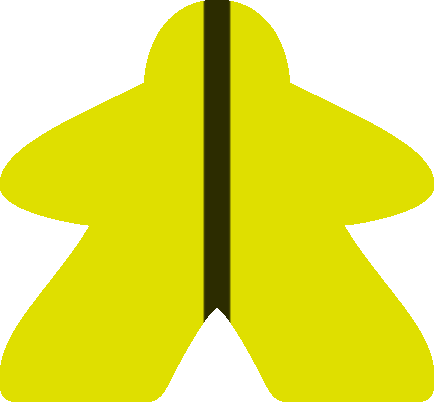
\includegraphics[scale=0.08]{meeples/meepleJaune_marqueur}, 
\includegraphics[scale=0.08]{meeples/meepleVert_marqueur}, 
\includegraphics[scale=0.08]{meeples/meepleViolet_marqueur})
\item 66x cartes recto-verso. Les cartes sont construites ainsi:
\begin{itemize}
\item[*] le verso 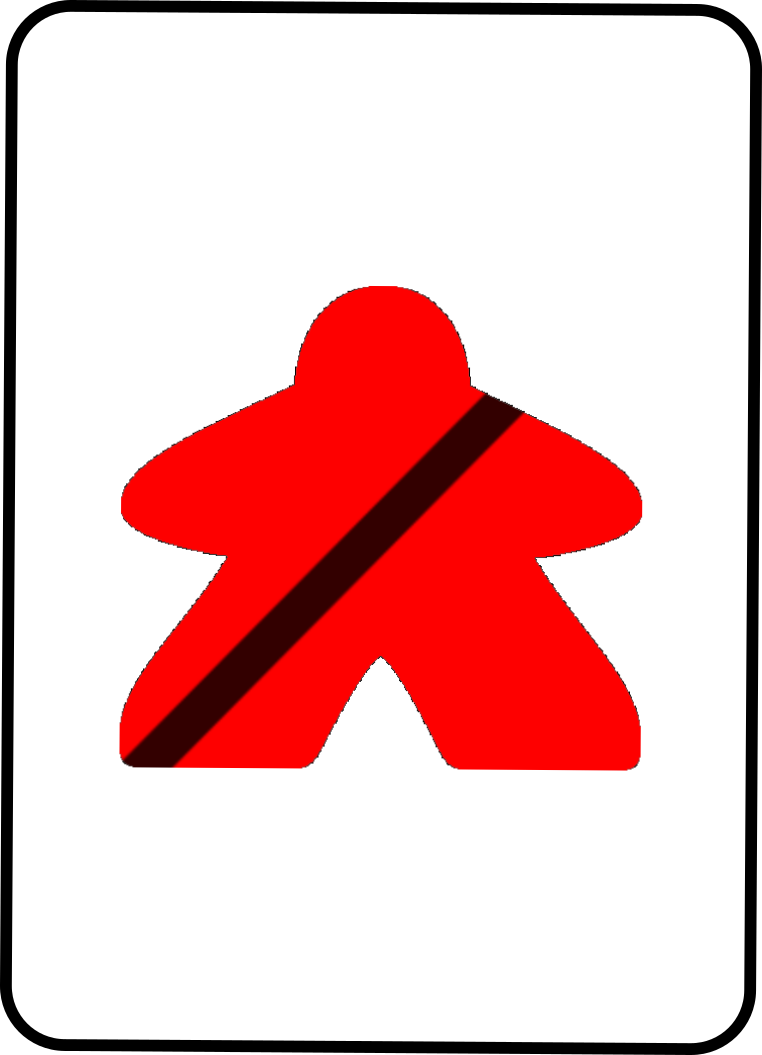
\includegraphics[scale=0.25]{regle/carteVerso} comporte un randonneur de couleur. Il permet d'indiquer le randonneur qui va se déplacer
\item[*] le recto 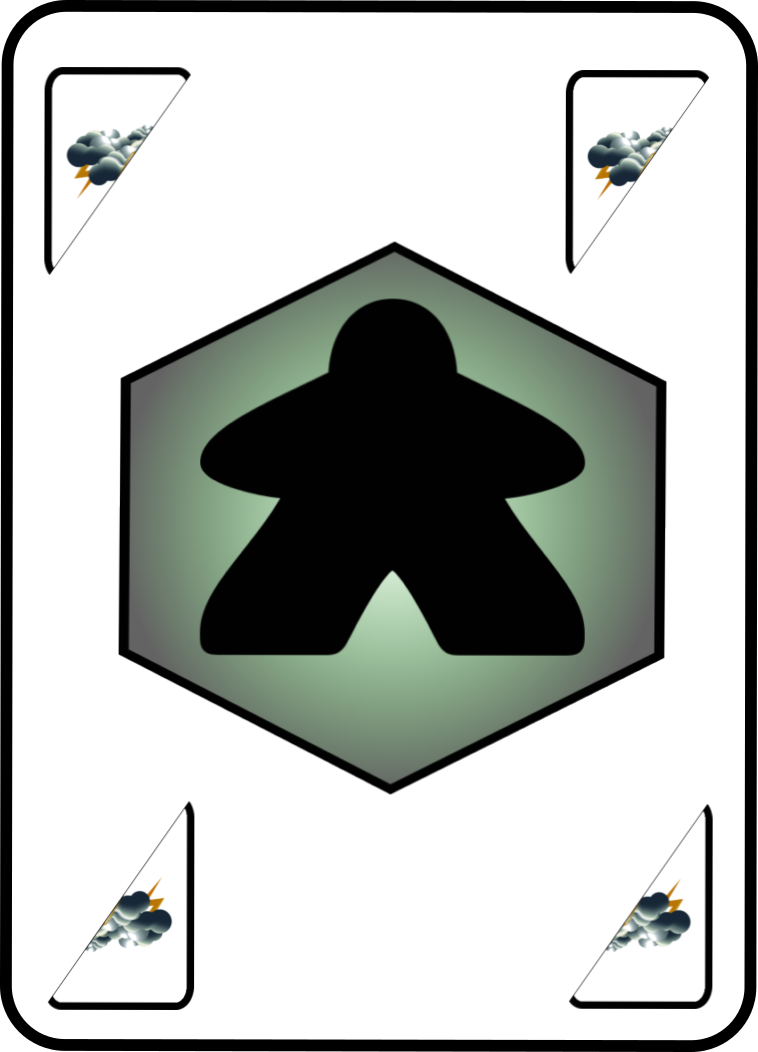
\includegraphics[scale=0.25]{regle/carteRecto} comporte deux informations: au centre, l'effet immédiat et dans les coins les informations de points en fin de partie.
\end{itemize}
\item un plateau central, divisé en plusieurs zones.
\end{itemize}

De plus, chaque joueur possède:
\begin{itemize}
\item un plateau pour indiquer les multiplicateurs d'actions.
\item 9 jetons de son esprit
\item 6 tuiles recto-verso 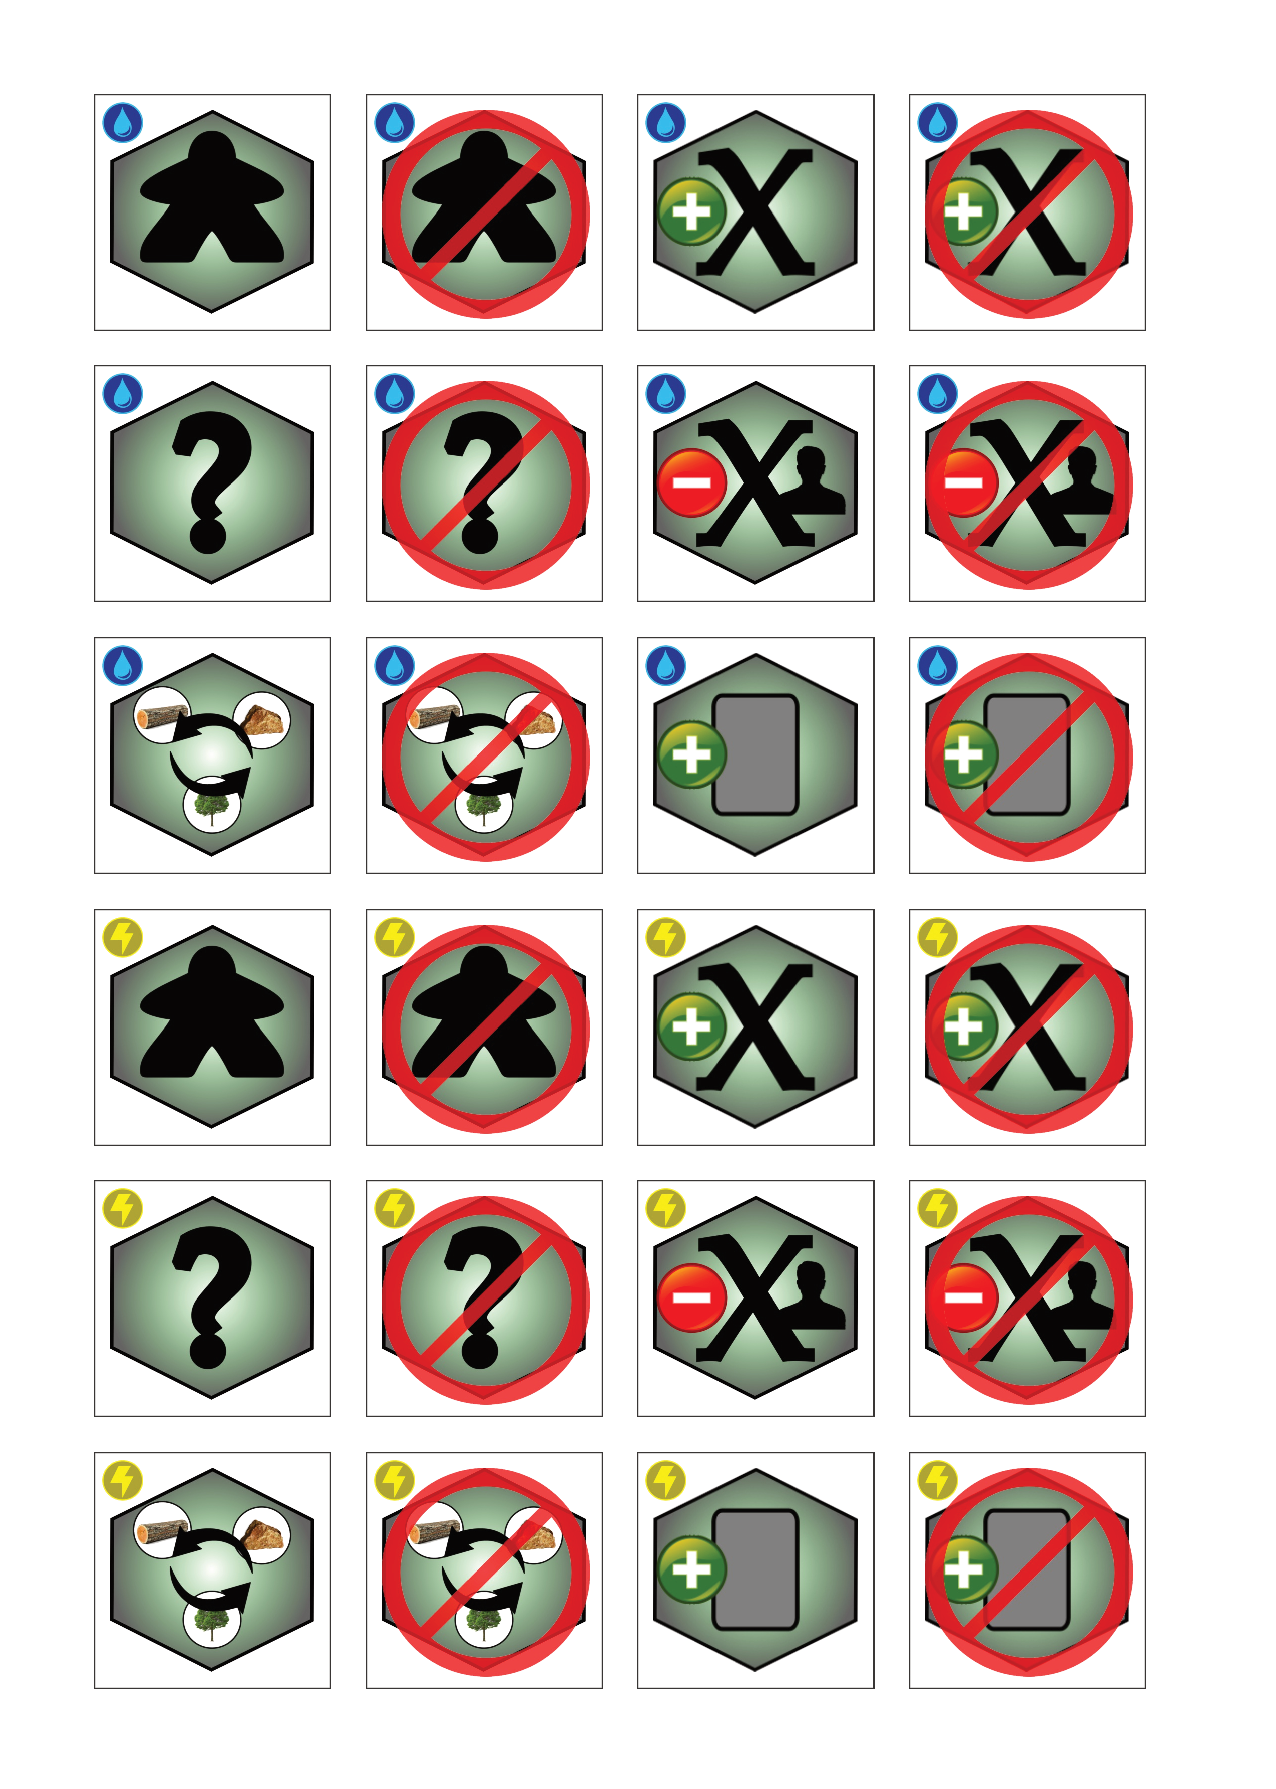
\includegraphics[scale=0.25]{regle/tuiles}, une pour chaque action possible. D'un côte, l'action est accessible (\tuileActive), de l'autre l'action est bloquée (\tuileBloquee).
\end{itemize}

\remarque{
Afin de faciliter la lecture pour les personnes atteintes d'altération de la perception des couleurs, tous les éléments de couleurs ont aussi un symbole.

\begin{tabular}{cc}
\text{\textbf{Couleur}} & \text{\textbf{Symbole}} \\ 
  \hline
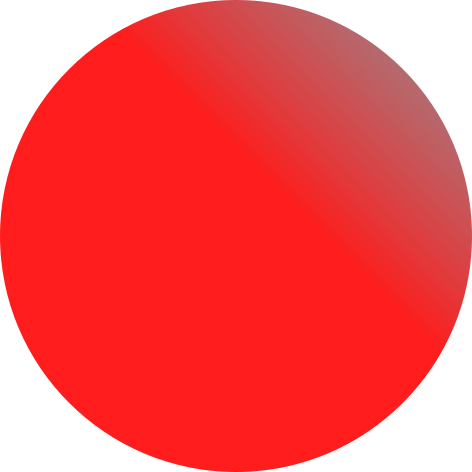
\includegraphics[scale=0.25]{obstacles/fond_rouge} &  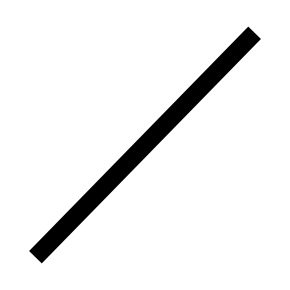
\includegraphics[scale=0.5]{marqueursCouleur/forme_forme1} \\ 
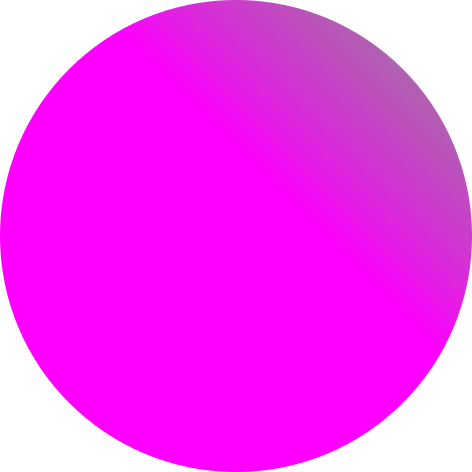
\includegraphics[scale=0.25]{obstacles/fond_violet} & 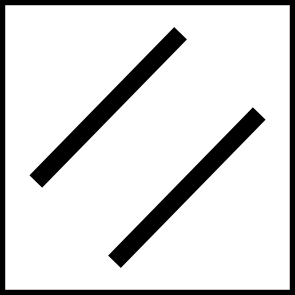
\includegraphics[scale=0.5]{marqueursCouleur/forme_forme2} \\ 
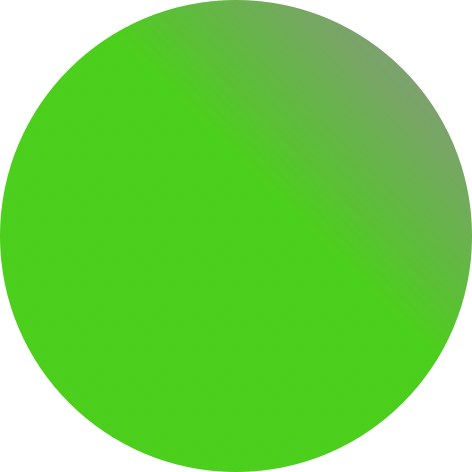
\includegraphics[scale=0.25]{obstacles/fond_vert} &  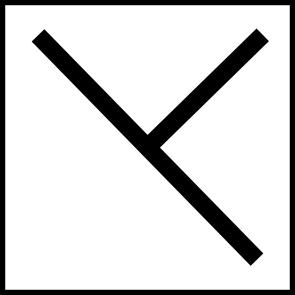
\includegraphics[scale=0.5]{marqueursCouleur/forme_forme3} \\ 
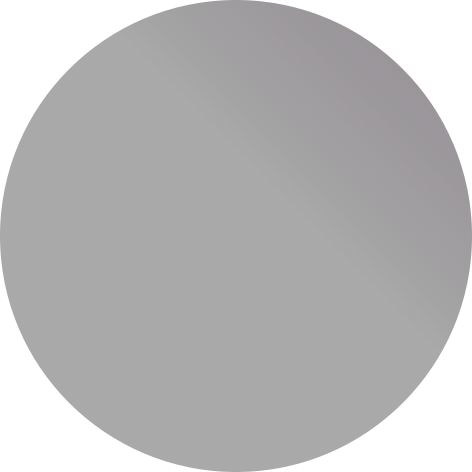
\includegraphics[scale=0.25]{obstacles/fond_gris} &  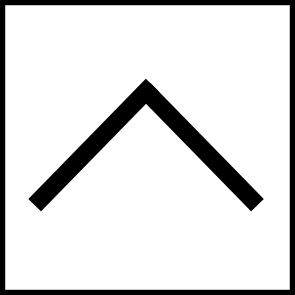
\includegraphics[scale=0.5]{marqueursCouleur/forme_forme4} \\
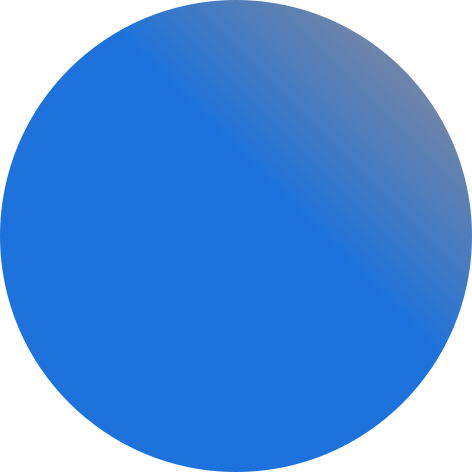
\includegraphics[scale=0.25]{obstacles/fond_bleu} &  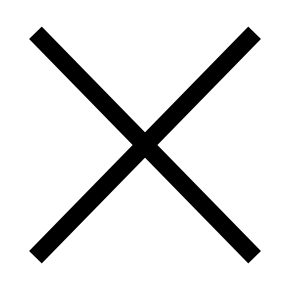
\includegraphics[scale=0.5]{marqueursCouleur/forme_forme5} \\ 
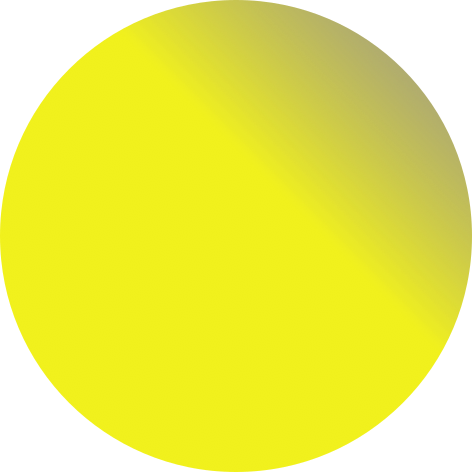
\includegraphics[scale=0.25]{obstacles/fond_jaune} &  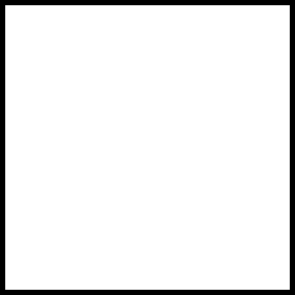
\includegraphics[scale=0.5]{marqueursCouleur/forme_forme6}  
\end{tabular} }
\FloatBarrier
